\documentclass[11pt,a4paper]{article}
\usepackage[utf8]{inputenc}
\usepackage[T1]{fontenc}
\usepackage{amsmath,amssymb}
\usepackage{graphicx}
\usepackage{booktabs}
\usepackage{natbib}
\usepackage{hyperref}
\usepackage{geometry}
\usepackage{caption}
\usepackage{setspace}
\usepackage{array}
\usepackage{microtype}

\geometry{margin=2.3cm}
\hypersetup{colorlinks=true,linkcolor=blue,citecolor=blue,urlcolor=blue}
\setstretch{1.08}
\emergencystretch=2em
\captionsetup{font=small,labelfont=bf}

\title{How Low-Dimensional Is the S--T--AOU Dependence of Ocean Total Dissolved Inorganic Carbon? A Symbolic Regression Analysis}
\author{Anonymous manuscript}
\date{}

\newcommand{\tco}{\mathrm{TCO_2}}
\newcommand{\aou}{\mathrm{AOU}}
\newcommand{\umol}{\,\mu\mathrm{mol}\,\mathrm{kg}^{-1}}

\begin{document}
\maketitle

\begin{abstract}
We quantify how much of the empirical dependence of ocean total dissolved inorganic carbon ($\tco$) on salinity ($S$), temperature ($T$), and apparent oxygen utilisation ($\aou$) can be represented by a compact nonlinear model. We analyze 472,530 quality-controlled GLODAP v2.2023 observations assigned to the Atlantic, Indian, Pacific, and Southern Ocean, and compare predefined linear, rank-1 quadratic, rank-2 quadratic, full quadratic, and cubic models with a symbolic-regression library generated by 48 searches across four operator spaces and three random seeds. The principal compact model, $\tco=(\alpha S+\beta T+\gamma\aou/100+\delta)^2+\epsilon$, has five fitted parameters. Its temporal-validation RMSE is 20.172, 14.483, 16.002, and 10.575~$\umol$ in the four basins, respectively. Adding a second squared projection changes RMSE by +1.984, +0.254, $-0.289$, and $-0.035~\umol$, providing no consistent predictive improvement. More flexible symbolic expressions reduce validation RMSE by approximately 3--12\% but have expression complexities of 15--25 versus 8 for rank-1. Rank-1 candidates occur in 24 of 48 search cells, although recovery depends on the operator space. Spatial-, cruise-, and post-2018 evaluations show generally useful transfer with basin-dependent rankings. Antarctic Intermediate Water is a high-error regime (rank-1 RMSE 28.426~$\umol$, bias +27.143~$\umol$), and a basin-scale Southern Ocean fit fails in the abyss while a local refit performs substantially better. These results support substantial empirical compressibility, but not a universal equation or a one-dimensional physical description of ocean carbon dynamics.
\end{abstract}

\noindent\textbf{Keywords:} total dissolved inorganic carbon; symbolic regression; rank-1 quadratic; GLODAP; model complexity; ocean carbon

\section{Introduction}

Total dissolved inorganic carbon ($\tco$) is a central observable for quantifying ocean carbon storage, air--sea carbon dioxide exchange, and biogeochemical change \citep{Sarmiento2006,Takahashi1993,Key2004}. Because observations are uneven in space and time, empirical relationships between $\tco$ and hydrographic or biogeochemical variables are used for interpolation, quality control, and regional carbon assessment. Salinity, temperature, and apparent oxygen utilisation are particularly attractive predictors because they summarize water-mass properties and remineralization history, but their joint relationship with $\tco$ is nonlinear and varies across the ocean \citep{Goyet1991,Millero1998,Broullon2019}.

Symbolic regression searches over mathematical expressions while retaining an explicit functional form \citep{Cranmer2023}. Here it is used as a probe of empirical compressibility, not as a mechanism-discovery procedure. We ask how much predictive structure can be retained when the dependence of $\tco$ on salinity ($S$), temperature ($T$), and apparent oxygen utilisation ($\aou$) is constrained to a single quadratic projection. The principal model is a squared affine projection with five fitted coefficients. We compare it with a second-rank quadratic extension, unconstrained polynomial families, and symbolic candidates over multiple operator spaces.

The analysis is designed to separate three questions that are often conflated. First, does a compact model predict substantially better than a linear baseline? Second, does increasing quadratic rank improve prediction under temporal, spatial, cruise, or external evaluation? Third, do compact structures transfer across basins and hydrographic regimes? A mathematical rank-1 Hessian answers only the first part of the structural question; it does not establish that ocean carbon dynamics have one physical degree of freedom. Accordingly, we interpret the fitted surface as an empirical approximation and treat its failure regimes as part of the result.

\section{Data and Methods}

\subsection{Observations, quality control, and basin assignment}
We used GLODAP v2.2023 observations of salinity, in situ temperature, apparent oxygen utilisation, and total dissolved inorganic carbon, together with latitude, longitude, depth, year, region, cruise, and station metadata \citep{Lauvset2023}. The primary-variable filters were strict: $25<S<42$, $-2.5<T<35\,^{\circ}\mathrm{C}$, $1700<\tco<2600\umol$, and $\aou>-50\umol$, with finite values required for all four modeled variables. These filters retained 512,384 rows. Basin-specific analyses used the 472,530 rows assigned to one of four mutually exclusive categories: Atlantic (region 1 and latitude $\geq-35^{\circ}$), Indian (region 16 and latitude $\geq-35^{\circ}$), Pacific (region 8 and latitude $\geq-35^{\circ}$), and Southern Ocean (latitude $<-35^{\circ}$). The remaining 39,854 QC-passing rows had no assignment to these four named basins and were excluded from basin-specific model fitting; this accounting explains why the full QC count differs from the main-analysis total. The basin and temporal counts are given in Table~\ref{tab:sample_sizes}.

For the rank-constrained and symbolic models, apparent oxygen utilisation was represented as $\aou_{100}=\aou/100$. This is a numerical scaling convention, not a change of units in the observations. Complete polynomial benchmarks were fitted using the implementation's corresponding polynomial basis; rescaling a predictor changes coefficients but not the span of a complete polynomial family.

\begin{table}[htbp]
\centering
\caption{Observations used in the four named-basin analyses. Training years are $<2015$; temporal validation years are 2015--2017; the external holdout is year $\geq2018$. The QC total includes 39,854 rows not assigned to a named basin.}
\label{tab:sample_sizes}
\small
\begin{tabular}{lrrrr}
\toprule
Basin & Total & Training & Validation & External \\
\midrule
Atlantic & 147,448 & 125,762 & 11,436 & 10,250 \\
Indian & 40,391 & 32,498 & 3,764 & 4,129 \\
Pacific & 187,443 & 138,202 & 31,791 & 17,450 \\
Southern Ocean & 97,248 & 82,045 & 6,483 & 8,720 \\
\midrule
Named-basin total & 472,530 & 378,507 & 53,474 & 40,549 \\
\bottomrule
\end{tabular}
\end{table}

\subsection{Temporal partitioning}
Observations with year $<2015$ were used for fitting. Observations from 2015 through 2017 formed the temporal validation set used for model comparison and symbolic-candidate selection. Observations from 2018 onward were reserved as a locked external holdout. No external-holdout result was used to select an expression, operator space, or model family.

\subsection{Model hierarchy}
The main comparison included a basin training-mean baseline, a linear model, two rank-constrained quadratic models, a full second-order polynomial, a full cubic polynomial, and frozen symbolic candidates. The rank-1 model was
\begin{equation}
\tco=(\alpha S+\beta T+\gamma\aou_{100}+\delta)^2+\epsilon,
\label{eq:rank1}
\end{equation}
with five fitted parameters. Its Hessian with respect to $(S,T,\aou_{100})$ is $2\mathbf{v}\mathbf{v}^{\mathsf T}$, where $\mathbf{v}=(\alpha,\beta,\gamma)^{\mathsf T}$, so the fitted model has quadratic rank one by construction.

The rank-2 model was
\begin{equation}
\tco=z_1^2+z_2^2+\epsilon,
\qquad z_j=a_jS+b_jT+c_j\aou_{100}+d_j,
\label{eq:rank2}
\end{equation}
with nine fitted parameters. No orthogonality, normalization, or canonical ordering constraint was imposed on the two coefficient vectors. Their decomposition is therefore rotationally non-identifiable, and the resulting quadratic form has rank at most two. Comparisons with rank-1 are consequently predictive comparisons between parameterizations, not tests of uniquely interpretable latent directions.

The full quadratic and cubic benchmarks contained 10 and 20 fitted coefficients, respectively. We distinguish fitted-parameter count $K$ from PySR expression complexity $C$, an expression-tree measure. The rank-1 model has $K=5$ and $C=8$. The hierarchy and temporal-validation results are summarized in Table~\ref{tab:model_performance}.

\begin{table}[htbp]
\centering
\caption{Temporal-validation RMSE by model family. RMSE is in $\mu\mathrm{mol}\,\mathrm{kg}^{-1}$. $K$ is the fitted-parameter count; $C$ is PySR expression complexity where defined.}
\label{tab:model_performance}
\small
\begin{tabular}{lrrrrrr}
\toprule
Model & $K$ & $C$ & Atlantic & Indian & Pacific & Southern Ocean \\
\midrule
Mean baseline & 1 & 1 & 66.879 & 122.473 & 131.396 & 59.190 \\
Linear & 4 & 4 & 21.591 & 14.960 & 17.769 & 10.664 \\
Rank-1 quadratic & 5 & 8 & 20.172 & 14.483 & 16.002 & 10.575 \\
Rank-2 quadratic & 9 & 16 & 22.155 & 14.737 & 15.712 & 10.540 \\
Full quadratic & 10 & 20 & 23.406 & 13.729 & 15.504 & 10.461 \\
Cubic & 20 & 30 & 22.598 & 11.827 & 14.244 & 10.042 \\
\bottomrule
\end{tabular}
\end{table}

\subsection{Symbolic regression}
Symbolic regression used PySR with four operator spaces, three seeds (42, 123, and 456), and one search for each basin--operator--seed combination, for 48 completed searches. The completed runs used 20 populations, population size 40, 50 iterations, maximum expression size 25, deterministic serial execution, and at most 30,000 training observations per run. Candidates were generated from training data, evaluated on the 2015--2017 validation set, and selected by validation RMSE, with complexity used to break ties. The post-2018 holdout remained locked.

The resulting library contains 599 raw, non-deduplicated candidate rows. A heuristic syntax-based classifier identified 86 rows as rank-1 quadratic candidates; this is a recurrence diagnostic, not a count of unique algebraic expressions. Pareto frontiers were computed from validation RMSE and expression complexity. Operator spaces differed in their ability to recover the rank-1 form, so recurrence is reported by search cell rather than treated as operator-invariant.

\subsection{Blocked validation and regional diagnostics}
Spatial generalization was evaluated with GroupKFold over $5^{\circ}$ latitude by $10^{\circ}$ longitude blocks, and sampling-event generalization with GroupKFold over available cruise identifiers. Both procedures used pre-2018 observations and maintained group disjointness between training and held-out folds. We also evaluated depth bins and threshold-based Atlantic water-mass classes. These classes are simplified screening categories rather than definitive hydrographic identifications. Finally, we compared the globally fitted Southern Ocean rank-1 model with a local refit for abyssal observations below 3000 m and colder than $1\,^{\circ}\mathrm{C}$.

\section{Results}

\subsection{Primary model comparison}
The regenerated temperature--salinity overview (Figure~\ref{fig:data_overview}) contains nonzero observations in all four named basins. The rank-1 model improved on the linear model in all four basins (Table~\ref{tab:model_performance}). Its temporal-validation RMSE was 20.172, 14.483, 16.002, and 10.575~$\umol$ in the Atlantic, Indian, Pacific, and Southern Ocean, respectively. The rank-2 minus rank-1 changes were +1.984, +0.254, $-0.289$, and $-0.035~\umol$ in the same order. Thus, adding four fitted parameters did not yield a consistent predictive improvement: rank-2 was worse in the Atlantic and Indian, and its improvements in the Pacific and Southern Ocean were small.

The full quadratic was less accurate than rank-1 in the Atlantic but improved slightly in the other three basins (Table~\ref{tab:model_performance}). Cubic models reduced validation RMSE further in the latter three basins, particularly the Indian, but used four times as many fitted coefficients. Figure~\ref{fig:model_hierarchy} shows the accuracy--complexity hierarchy.

\begin{figure}[htbp]
\centering
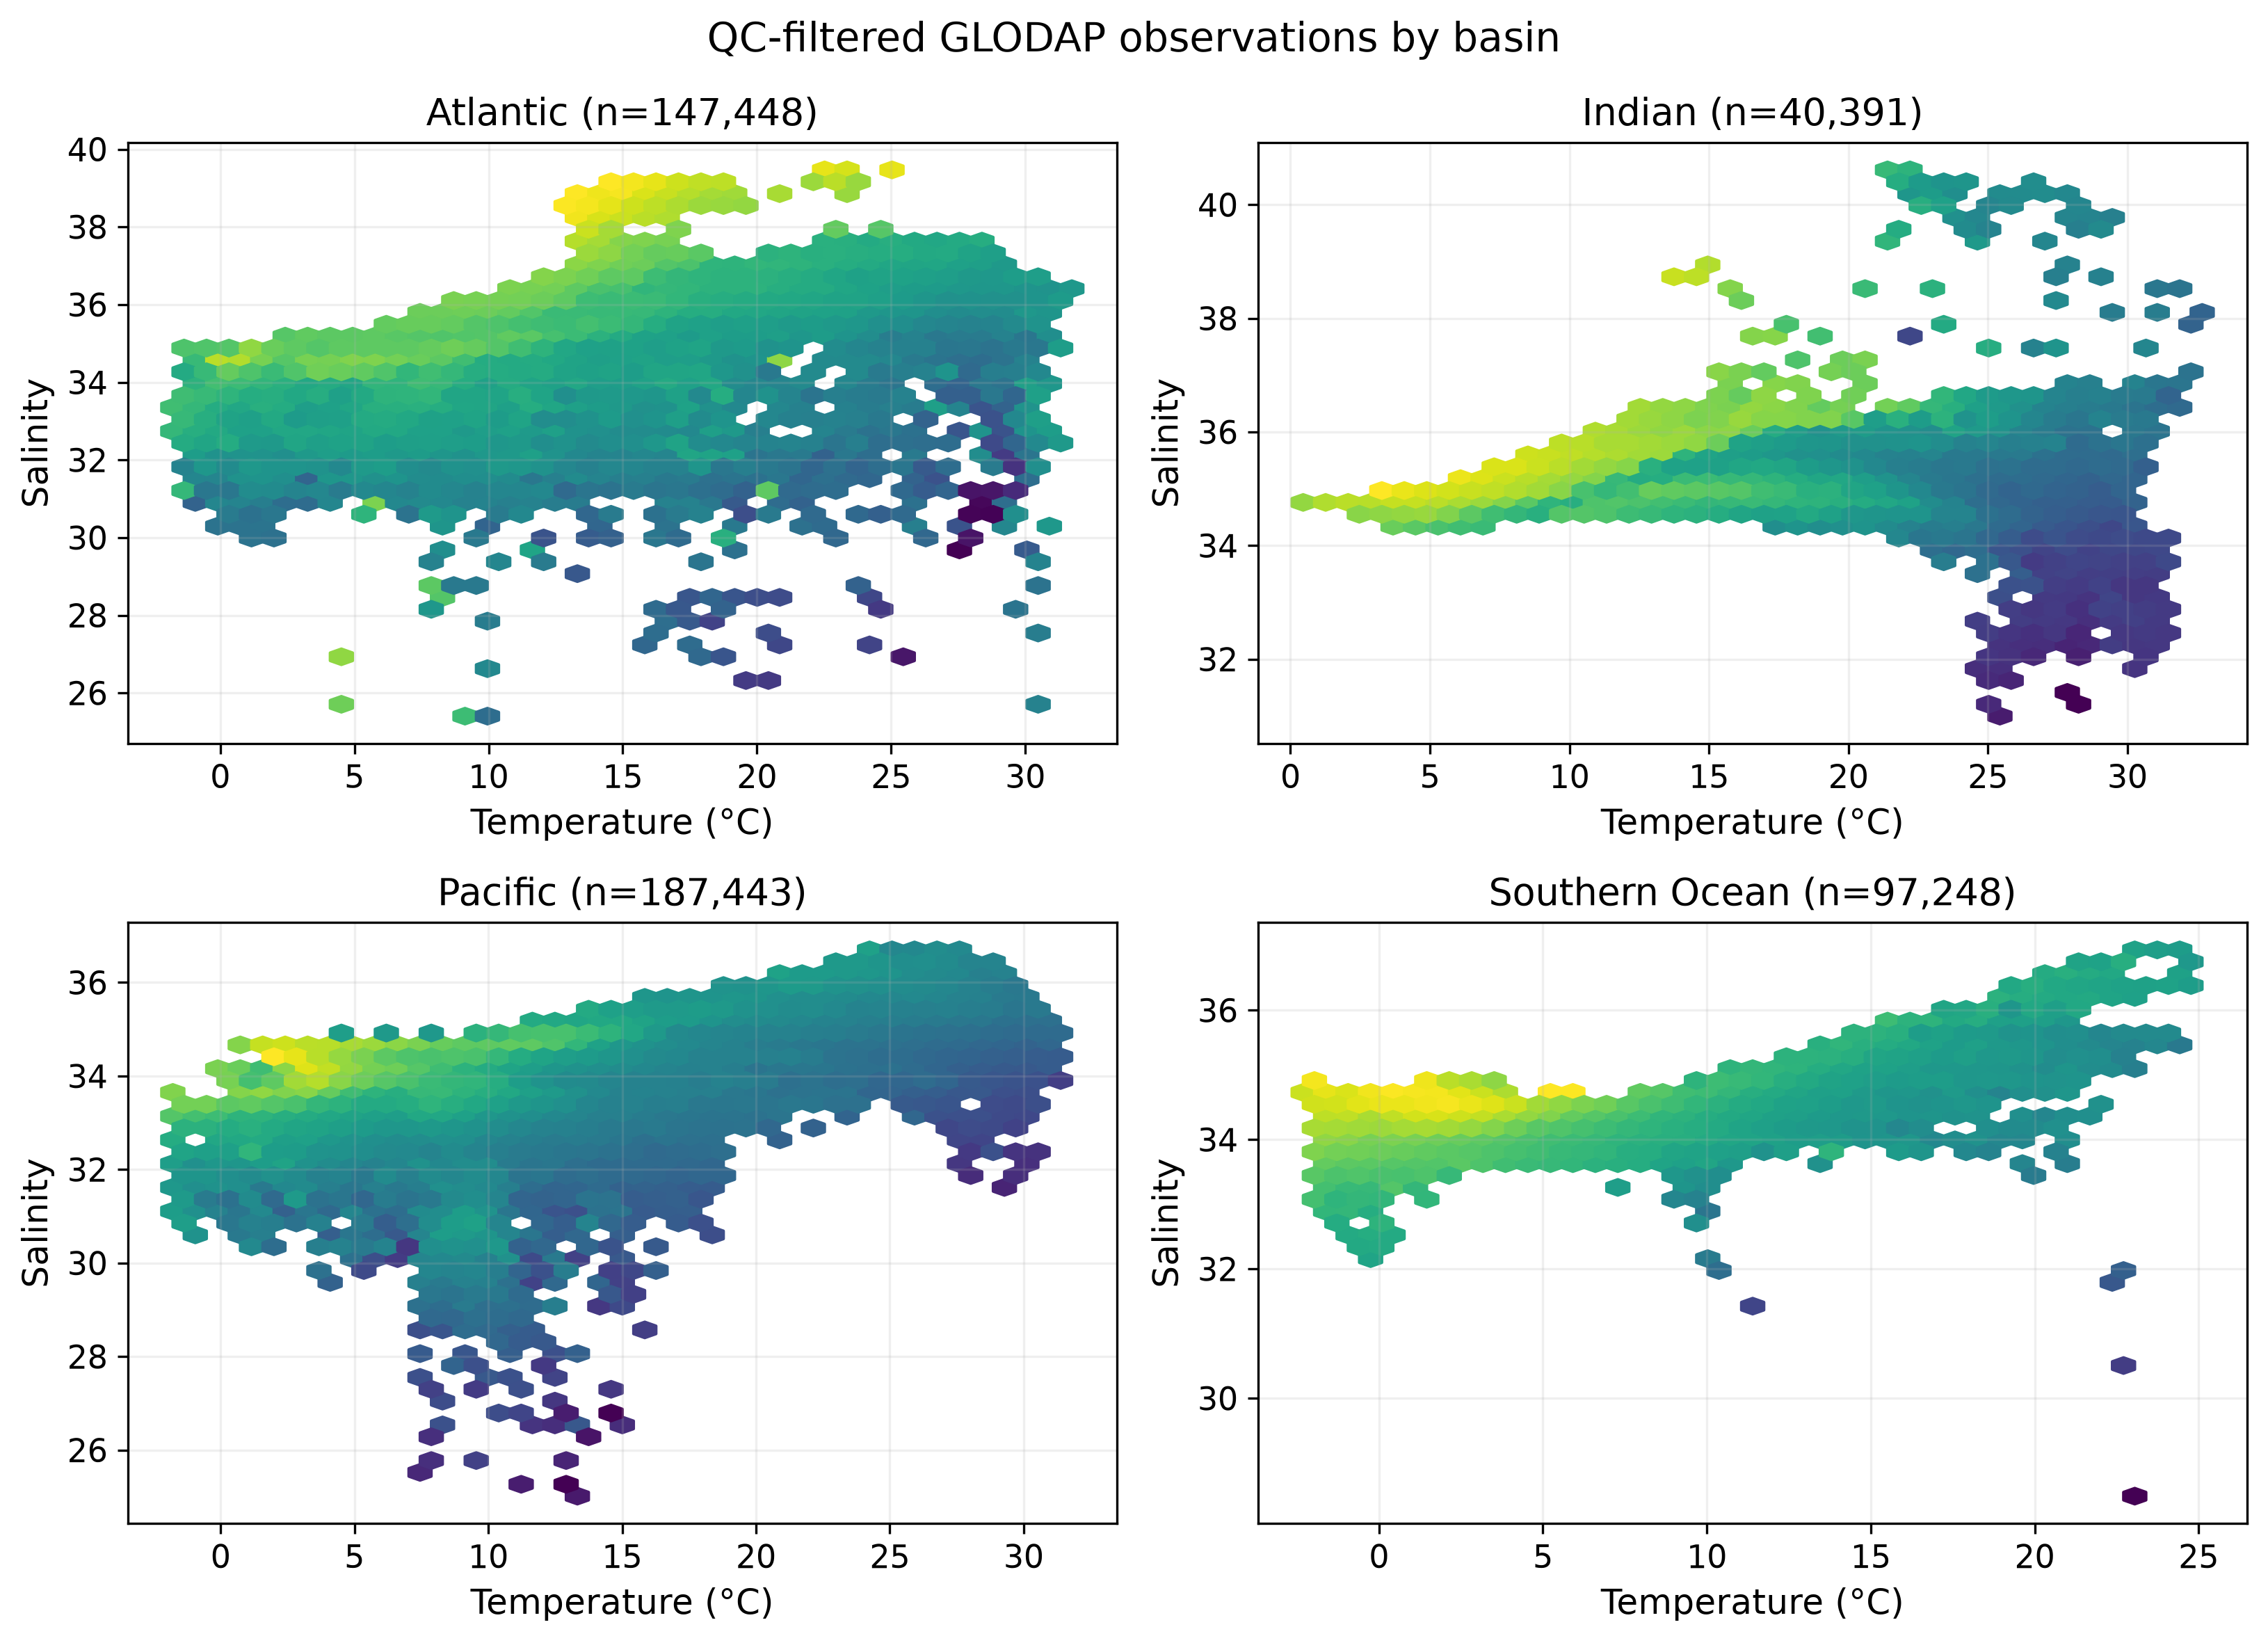
\includegraphics[width=\textwidth]{figures/figure1_data_overview.png}
\caption{Quality-controlled GLODAP observations in temperature--salinity space, colored by measured $\tco$. Panel counts are the four named-basin totals used in the analysis.}
\label{fig:data_overview}
\end{figure}

\begin{figure}[htbp]
\centering
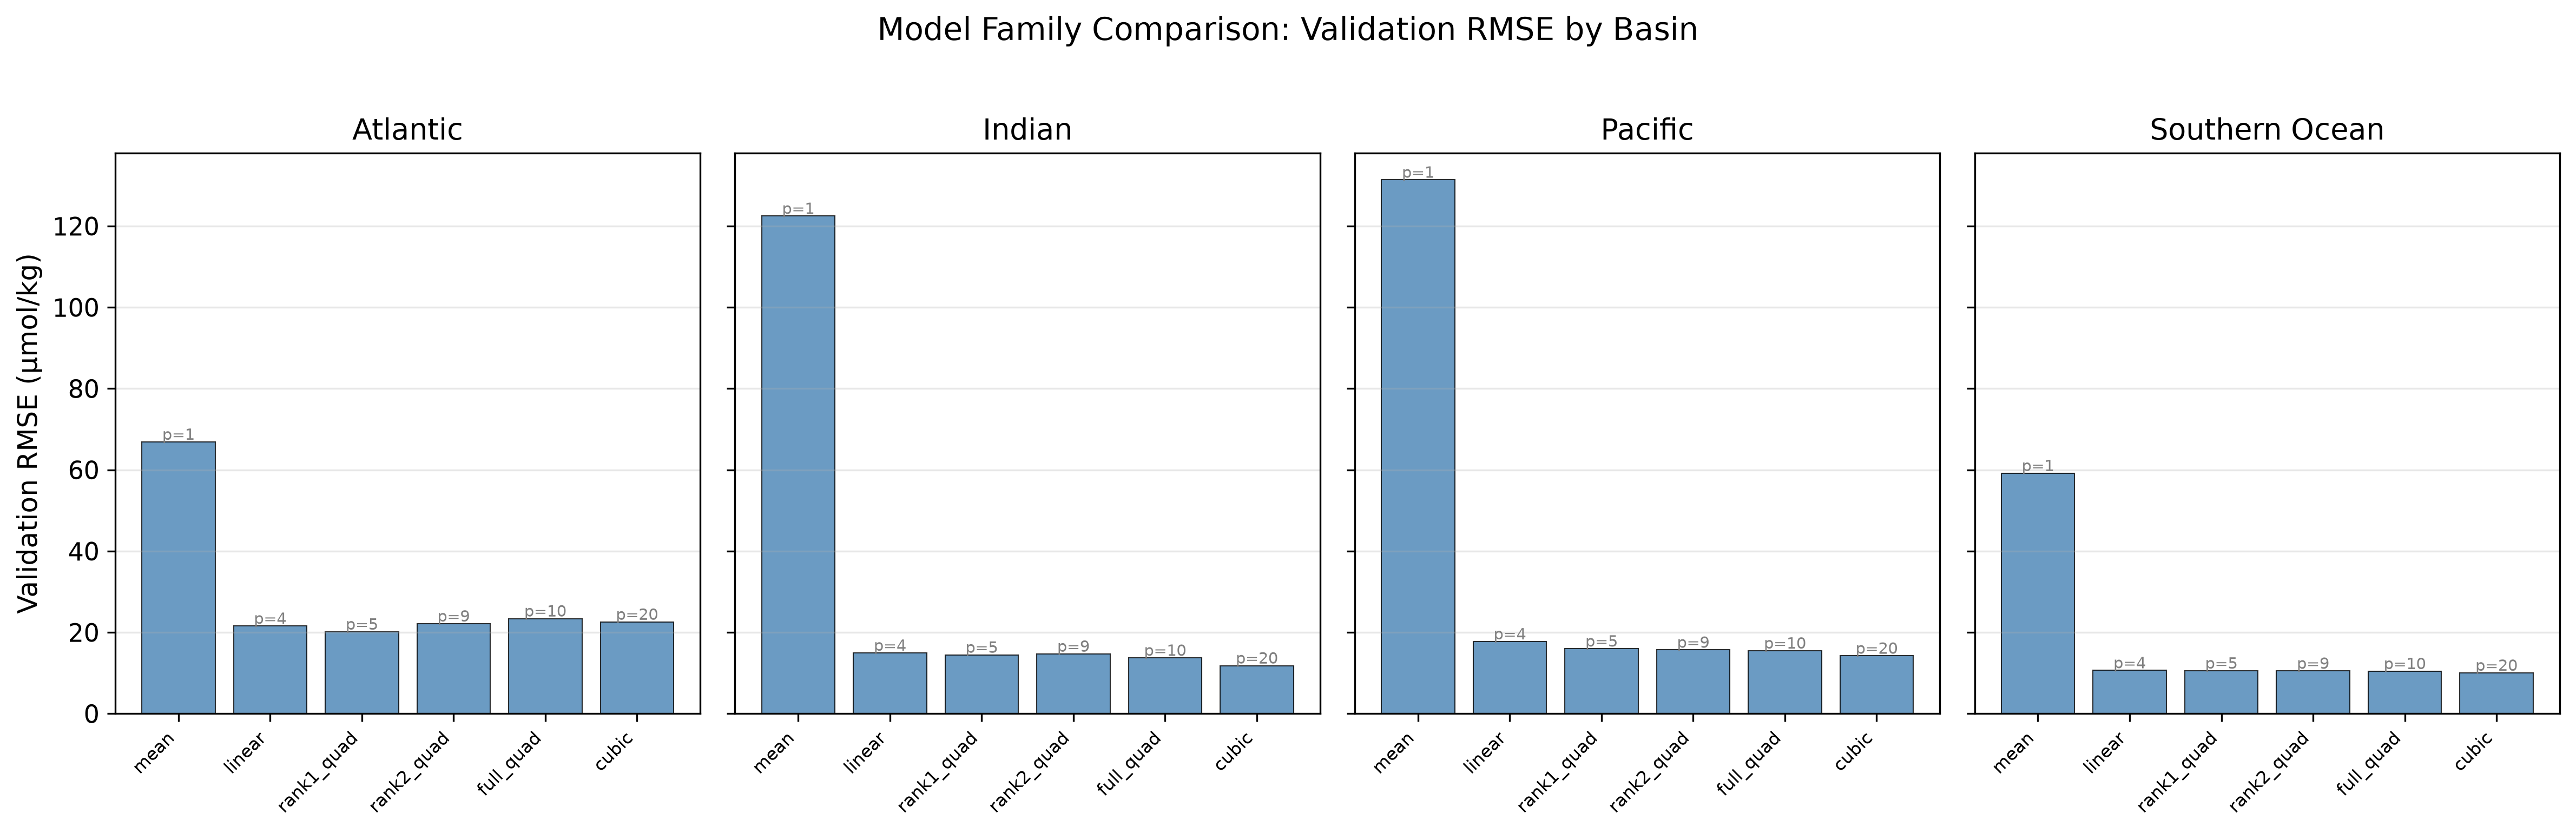
\includegraphics[width=\textwidth]{figures/figure2_model_hierarchy.png}
\caption{Temporal-validation RMSE for the predefined model families. Parameter counts are annotated in the source figure. The rank-1 model improves on the linear model in all basins but is not uniformly the most accurate family.}
\label{fig:model_hierarchy}
\end{figure}

\subsection{Symbolic recurrence and accuracy--complexity trade-off}
Rank-1 candidates occurred in 24 of 48 basin--operator--seed cells and in all four basins. Recovery was not operator-invariant: in the Atlantic, rank-1 candidates appeared only in the search space containing an explicit square operator. The count of 86 rank-1-classified rows includes repeated and syntactically classified candidates, so it should not be interpreted as 86 independent discoveries.

The best symbolic candidates improved validation RMSE relative to rank-1 by approximately 5.8\% in the Atlantic, 11.6\% in the Indian, 3.2\% in the Pacific, and 5.6\% in the Southern Ocean. Their complexities were 15, 25, 20, and 21, compared with $C=8$ for rank-1. Figure~\ref{fig:pareto} shows the trade-off: the compact model occupies the low-complexity end, while more complex expressions can improve accuracy. Rank-1 is therefore an efficient approximation rather than a universally preferred model.

\begin{figure}[htbp]
\centering
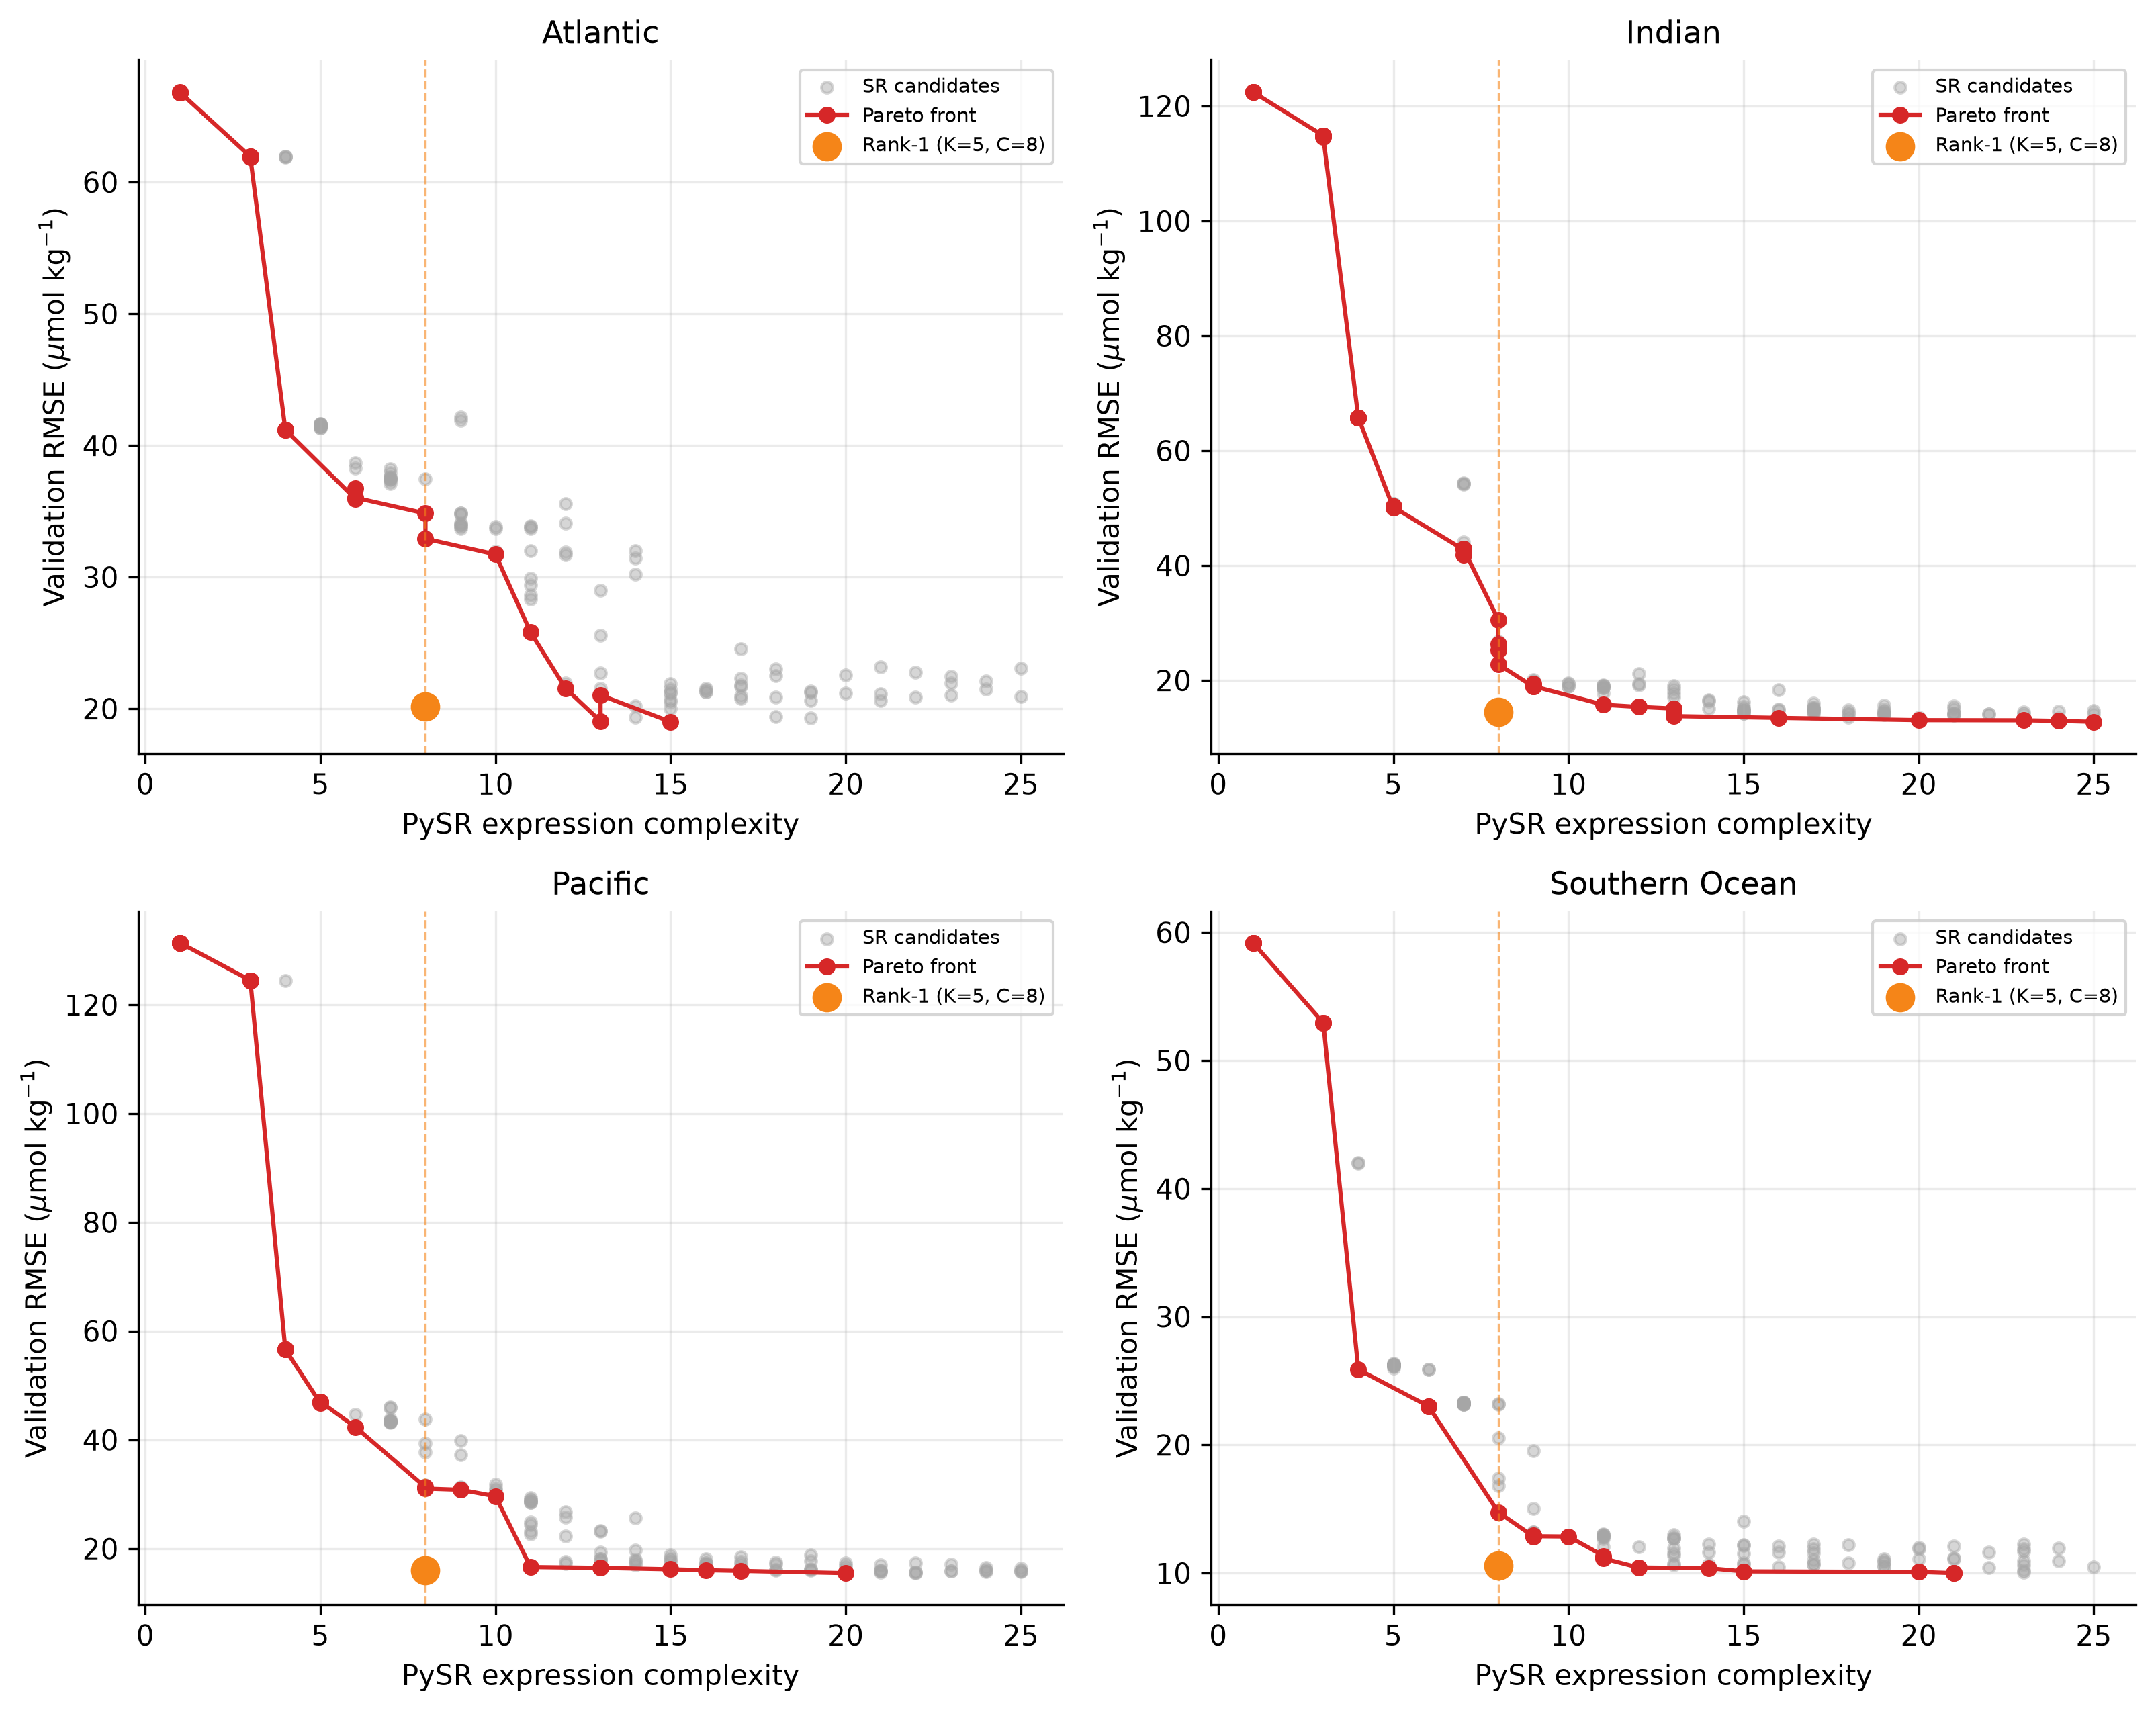
\includegraphics[width=0.9\textwidth]{figures/figure3_pareto_frontier.png}
\caption{Symbolic-regression validation RMSE versus PySR expression complexity. The vertical reference marks the rank-1 complexity ($C=8$). Higher-complexity candidates can reduce error, but expression complexity and fitted-parameter count are distinct quantities.}
\label{fig:pareto}
\end{figure}

\subsection{Temporal, spatial, cruise, and external generalization}
Table~\ref{tab:generalization} summarizes rank-1 performance across validation regimes. Spatial-block RMSE was 16.299, 16.609, 16.031, and 9.157~$\umol$ across the four basins; cruise-block RMSE was 16.910, 17.394, 16.031, and 9.225~$\umol$. Rankings changed across schemes: for example, in Atlantic spatial validation, rank-2 and full quadratic outperformed rank-1 even though rank-1 was better under the primary temporal split.

The locked post-2018 results support temporal transfer within the sampled distribution (Table~\ref{tab:generalization}). Neither blocked design establishes arbitrary geographic extrapolation.

\begin{table}[htbp]
\centering
\caption{Selected regional diagnostics. Water-mass values are from the Atlantic temporal-validation subset; abyssal values compare a global Southern Ocean fit with a local abyssal refit.}
\label{tab:regional}
\small
\begin{tabular}{llrrrr}
\toprule
Regime & Model & $N$ & RMSE & Bias & $R^2$ \\
\midrule
AAIW & Rank-1 & 428 & 28.426 & +27.143 & -0.115 \\
AAIW & Full quadratic & 428 & 22.333 & +21.126 & 0.312 \\
NADW & Rank-1 & 2,693 & 9.767 & -2.701 & 0.660 \\
Abyss, global & Rank-1 & 855 & 7.447 & +5.876 & -0.174 \\
Abyss, local refit & Rank-1 & 855 & 3.182 & --- & 0.786 \\
\bottomrule
\end{tabular}
\end{table}

\begin{table}[htbp]
\centering
\caption{Rank-1 RMSE across validation regimes. Spatial blocks are $5^{\circ}\times10^{\circ}$; cruise blocks use the available cruise identifier. Units are $\mu\mathrm{mol}\,\mathrm{kg}^{-1}$.}
\label{tab:generalization}
\small
\begin{tabular}{lrrrr}
\toprule
Basin & Temporal & Spatial block & Cruise block & External $\geq2018$ \\
\midrule
Atlantic & 20.172 & 16.299 & 16.910 & 17.672 \\
Indian & 14.483 & 16.609 & 17.394 & 18.413 \\
Pacific & 16.002 & 16.031 & 16.031 & 13.821 \\
Southern Ocean & 10.575 & 9.157 & 9.225 & 8.985 \\
\bottomrule
\end{tabular}
\end{table}

\begin{figure}[htbp]
\centering
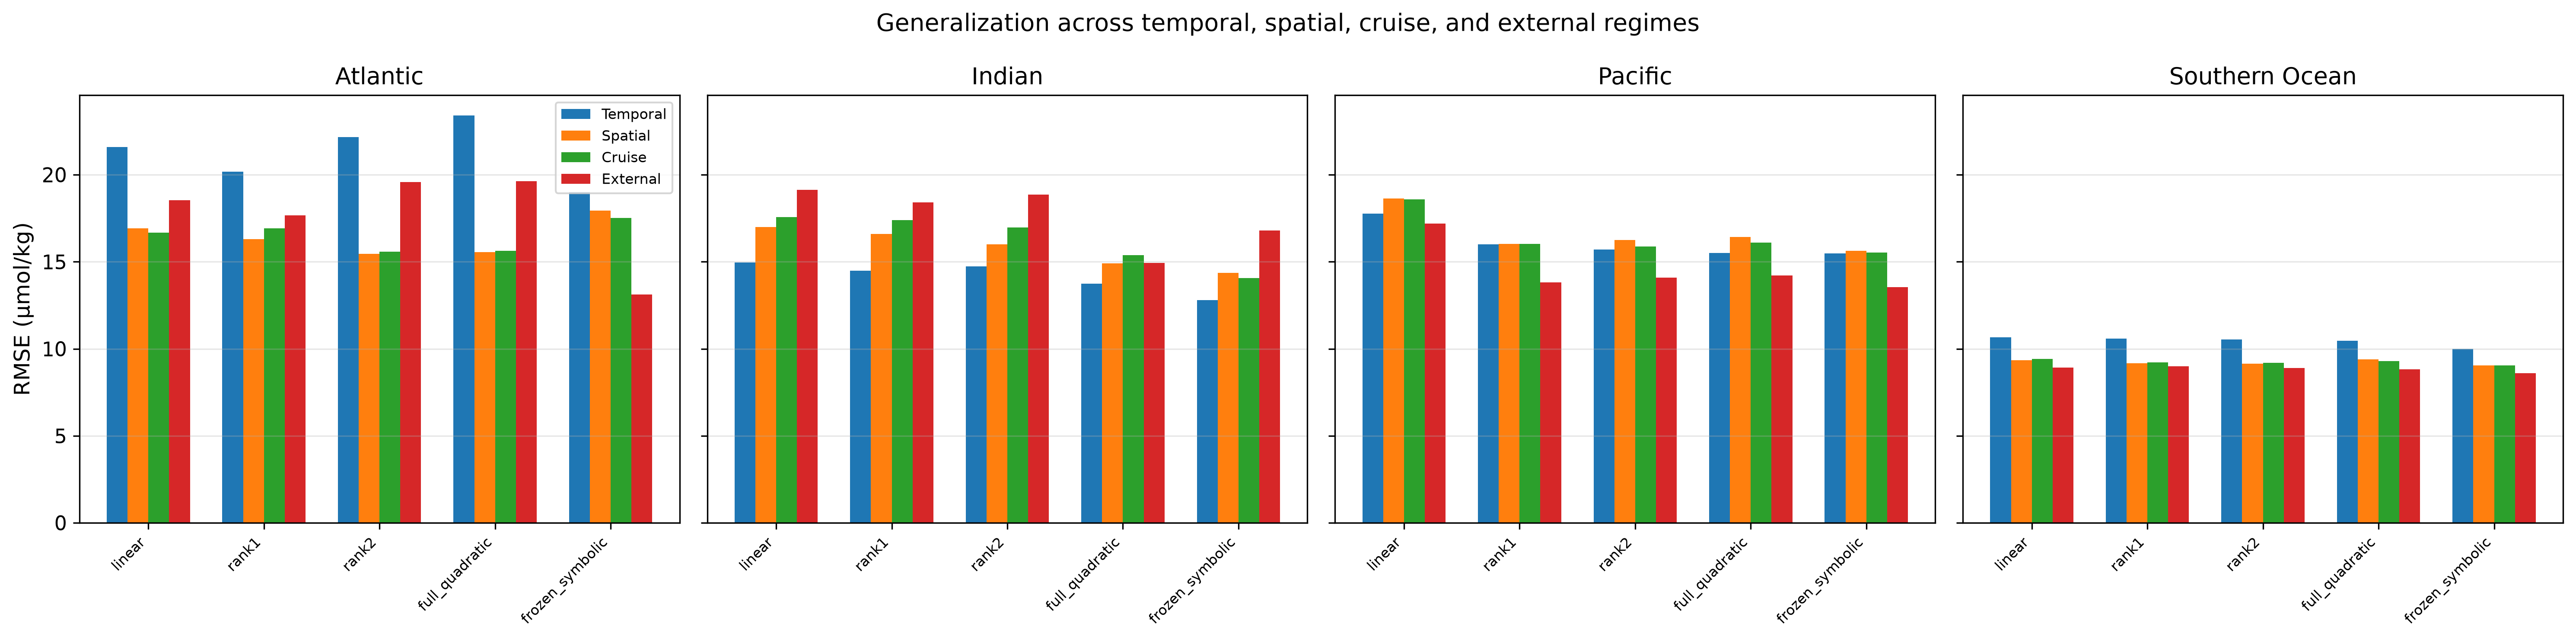
\includegraphics[width=\textwidth]{figures/figure4_generalization.png}
\caption{RMSE for linear, rank-1, rank-2, full-quadratic, and selected frozen symbolic models under temporal, spatial-block, cruise-block, and locked external evaluation. Rankings vary with validation regime.}
\label{fig:generalization}
\end{figure}

\subsection{Regional and water-mass limitations}
Errors were strongly regime-dependent. In the Atlantic threshold-based water-mass analysis, rank-1 RMSE was 28.426~$\umol$ with bias +27.143~$\umol$ for AAIW ($N=428$), whereas the full quadratic had RMSE 22.333~$\umol$ and bias +21.126~$\umol$. NADW was substantially better predicted by rank-1 (RMSE 9.767~$\umol$, bias $-2.701~\umol$, $N=2,693$). The contrasting AAIW and NADW results emphasize that basin-average performance does not describe all water-mass regimes.

The Southern Ocean abyss provides a sharper transferability test. For observations deeper than 3000 m and colder than $1\,^{\circ}\mathrm{C}$, the globally fitted rank-1 model had $R^2=-0.174$ and RMSE 7.447~$\umol$. A rank-1 model refit to the local abyssal training subset achieved $R^2=0.786$ and RMSE 3.182~$\umol$. The contrast is consistent with coefficient-transfer failure or domain shift; it does not show that abyssal $\tco$ is intrinsically unpredictable.

\begin{figure}[htbp]
\centering
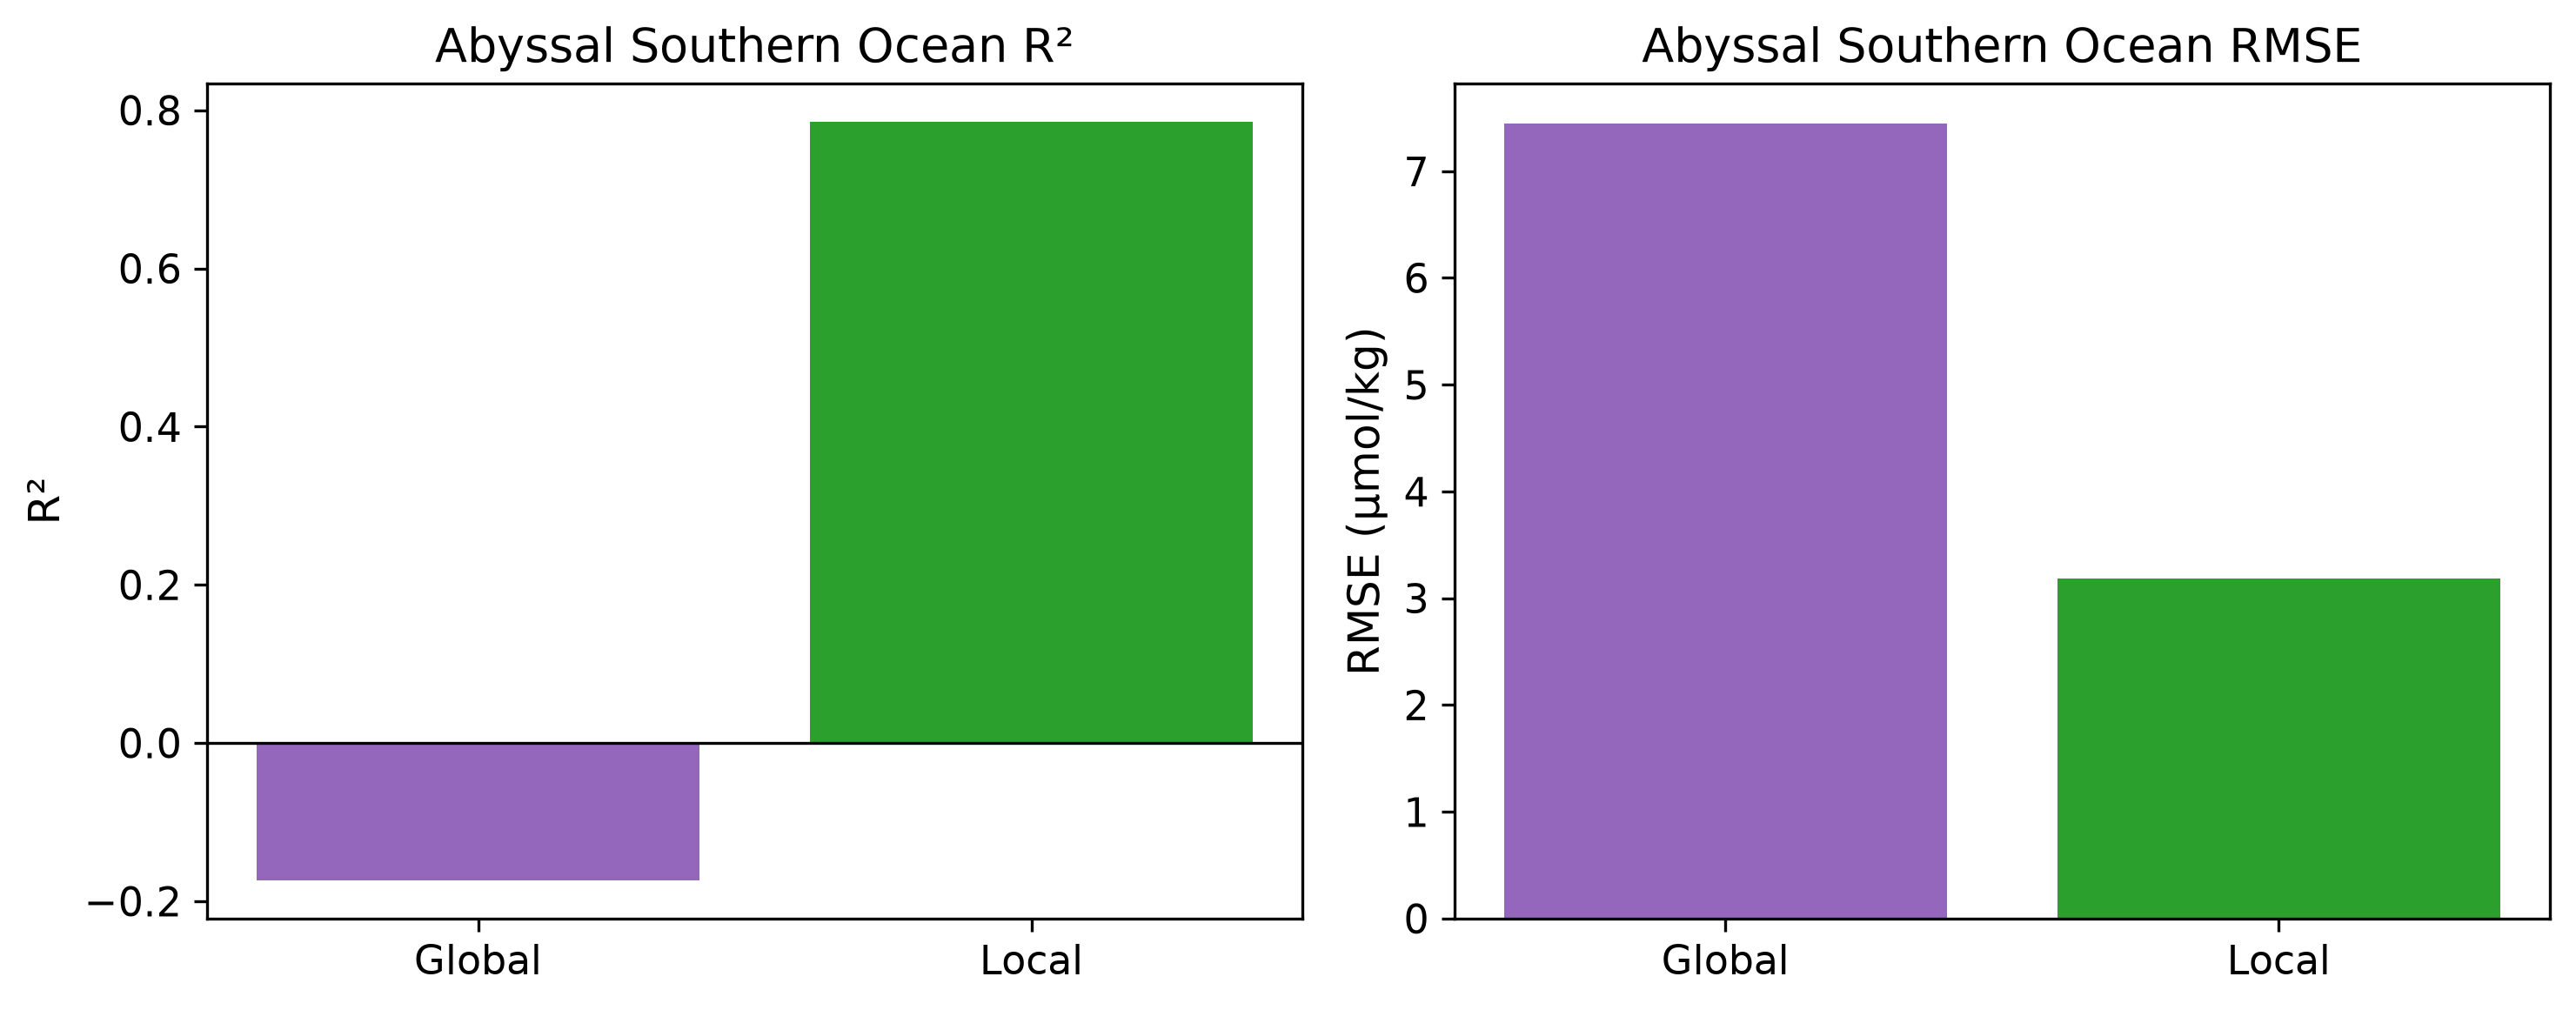
\includegraphics[width=0.8\textwidth]{figures/figure5_southern_abyss.png}
\caption{Southern Ocean abyssal performance for a basin-scale rank-1 fit and a local abyssal refit. The local improvement demonstrates domain dependence of the coefficients.}
\label{fig:abyss}
\end{figure}

\section{Discussion}

The results support substantial empirical compressibility of the $S$--$T$--$\aou$ dependence of $\tco$. A five-parameter squared projection improves on a linear model in all four basins and remains close to the full quadratic in three of them, while the rank-2 extension provides no consistent gain under temporal validation. This is useful evidence that a compact nonlinear approximation can retain much of the predictive signal in the sampled data.

The conclusion is deliberately narrower than a claim of one-dimensional ocean carbon dynamics. Rank-1 curvature is a property imposed by Equation~\ref{eq:rank1}; the rank-2 comparison evaluates predictive benefit, not the physical dimensionality of the carbon system. Likewise, recurrence in symbolic searches depends on the available operators, and the 24/48 cell recurrence rate is not evidence that the expression is uniquely selected by the data.

The accuracy--complexity results clarify why the rank-1 model remains scientifically useful even when more flexible candidates predict better. Symbolic candidates with complexities 15--25 reduce validation RMSE by 3--12\%, but the rank-1 model offers a transparent five-parameter baseline. Its practical value is therefore as a compact empirical parameterization and diagnostic benchmark, not as a universally optimal predictor.

Transferability is the principal limitation. Temporal, spatial-block, and cruise-block evaluations give different model rankings, and the AAIW and Southern Ocean abyss analyses show that basin-scale coefficients can fail in specific hydrographic regimes. Threshold-based water-mass classes are useful for locating these failures but do not replace neutral-density or endmember analyses. The locked post-2018 evaluation reduces one form of selection bias, yet the 2015--2017 validation period was used repeatedly for candidate selection and should not be treated as an independent test set.

Several methodological limitations also bound interpretation. Symbolic searches were restricted to predefined operator spaces and moderate effective search settings; the family classifier was syntactic and candidates were not fully algebraically deduplicated. GLODAP observations are clustered by cruise, station, and location, so observation-level uncertainty calculations require care. We therefore make no formal claim of universal equivalence between rank-1 and full quadratic models, and we do not interpret fitted derivative signs or Hessian rank as evidence of causality. The empirical result is strongest as a model-compression statement with explicitly characterized domain limits.

\section{Conclusions}

Across 472,530 named-basin GLODAP v2.2023 observations, the empirical dependence of $\tco$ on salinity, temperature, and apparent oxygen utilisation was substantially compressible into a five-parameter rank-1 quadratic projection. The model improved on a linear baseline in every basin, and adding a second squared projection produced no consistent validation benefit. More complex symbolic expressions achieved lower validation error, but at two- to three-fold greater expression complexity.

The compact structure was not invariant across symbolic operator spaces or validation regimes. Performance also depended on basin, depth, and water-mass context: AAIW showed large positive bias, and a globally fitted Southern Ocean model failed in the abyss while a local refit performed well. The appropriate conclusion is therefore an empirical and conditional one. Rank-1 quadratic structure is a useful low-complexity approximation for the sampled ocean-carbon relationship, but it is neither a universal predictor nor evidence that the physical dimensionality of ocean carbon dynamics is one.

\section*{Data and Code Availability}
GLODAP v2.2023 is publicly available through the Global Ocean Data Analysis Project. The analysis code, configuration files, processed result summaries, and figure-generation scripts accompany this manuscript. The raw GLODAP file is not redistributed here and remains subject to the provider's terms.

\section*{Acknowledgements}
We acknowledge the GLODAP data contributors, oceanographic cruise participants, and developers of PySR and SymbolicRegression.jl.

\section*{Competing Interests}
The authors declare no competing interests.


\bibliographystyle{apalike}
\bibliography{../references}

\end{document}
